% ---------------------- THESIS TEMPLATE ---------------------- %
%----------- Adapted by Samuel B. Kachuck, '10 ------------- %
%----------- from Joshua Bodyfelt '09's Ph.D. thesis --------- %

% --Instructions:
% This document is to be used as a template for a senior honors
% thesis in the physics department.  If you are at the point of using 
% this, unless you are a theorist, you're experiment is done, your 
% results discovered, and you are doing pretty well.  So the
% rest should be relatively simple, but still deserves exposition.  

% 1. Fill in the required parts of the title page.  This includes:
%	a. The title (make it good!)
%	b. Your name
%	c. Your class year
%	d. The date of submission (Month, Year)
% 2. Write your dedication and abstract in the files included
% 3. Write Chapters and include them.  This involves:
%	a. Creating a new .tex file that starts with (see example)
%			\pagestyle{empty}
%			\fancyhead[LO]{\leftmark}   
%			\chapter{A Sample Chapter for You!}
%			\label{ch:sample}
%			\pagestyle{fancy}
%			\graphicspath{{./ch1_sample/figs/}}
%	b. Saving the file in its own directory
%	c. Including it as a chapter below in the chapter inclusion
%		section in the same fashion as the example
% 4. Acknowledge those people that helped you (probably many 
%		more than initially expected)
% 5. Replace my bibliography with yours
%
% 6. Turn it in, and enjoy the rest of your year!
%
% For a good tutorial on LaTeX, see
% www.ctan.org/tex-archive/info/lshort/english/lshort.pdf
% or google "The Not So Short Introduction to LaTeX"

\documentclass[10pt,letterpaper, oneside]{book}
\usepackage{fancyhdr}  % enables use of fancy pagestyle
\usepackage[Lenny]{fncychap}
\usepackage{geometry} 
\usepackage{sidecap}
\usepackage{float}
\usepackage{mhchem}
\usepackage[parfill]{parskip}    % Activate to begin paragraphs with an empty line
\usepackage{graphicx}
\usepackage{subfig}
\usepackage{revsymb}
\usepackage{multirow}
\usepackage{wrapfig} 
\usepackage{amssymb}
\usepackage{amsmath}
\usepackage{mathrsfs} %required for \mathscr (prettiest calligraphic font for Lagrangian and FT)
\usepackage{verbatim}
\usepackage{color}
\usepackage{cite}
%\usepackage{here} %"!h" forces the graph to print here.  "!t" force the graph to typeset at top of page.
\usepackage{caption}
\captionsetup{font=footnotesize, labelfont=bf}

\DeclareGraphicsRule{.tif}{png}{.png}{`convert #1 `dirname #1`/`basename #1 .tif`.png}
\DeclareGraphicsExtensions{.pdf,.eps,.png,.jpg}
\textwidth 5.750in \textheight=8.000in \headheight 0.0625in \topmargin 0.228in % book strict
\oddsidemargin 0.500in \evensidemargin 0.500in 
%gs \oddsidemargin 0.563in \evensidemargin 0.2500in               %for two sided printing
\newcommand{\conditionalblankpage}{\cleardoublepage}  %for two sided printing 
%gs \newcommand{\conditionalblankpage}{}  %for doing nothing

\renewcommand{\baselinestretch}{1.5}
%%%%%%%%%%%%%%%%%%%%
\begin{document}
%%%%%%%%%%%%%%%%%%%%



%%%%%%%%%%%%%%%%%%%%

\pagenumbering{roman}
\pagestyle{empty} 
\begin{titlepage}
\begin{center}
\rule{5.75in}{1pt} \\
\vspace*{-0.125in}
{\large Wesleyan University} \hfill {\large Physics Department}
\rule[0.2in]{5.75in}{1pt} \\
\vspace*{1.1in}
{\LARGE \bf Generic Title} \\					% a. THE TITLE
\vspace*{0.05in}
\vspace*{0.25in}
{\Large by \\ \vspace*{0.10in}  Your Name Here\\ Class of \\}  % b., c., YOUR NAME AND CLASS YEAR
\vspace*{1.25in}
{\large An honors thesis submitted to the\\ faculty of Wesleyan University\\ in partial fulfillment of the requirements for the \\Degree of Bachelor of Arts \\ with Departmental Honors in Physics \vspace*{-0.15in} }\vspace*{.25in}
\rule{5.75in}{1pt} \\
\vspace*{-0.125in}
{\large Middletown, Connecticut \hfill April, 2010}		% d., THE DATE
\rule[0.2in]{5.75in}{1pt} \\
\end{center}
\end{titlepage}

\vspace*{0.95in}
{\Huge \bf Dedication}
\vspace*{0.5in}\\

Dedicate here

{\Huge \bf Abstract}
\vspace*{0.1in}\\

Abstract goes here.

\tableofcontents
\listoffigures 
\conditionalblankpage
\pagestyle{fancy}
\fancyhead{}
\renewcommand{\chaptermark}[1]{\markboth{Chapter \thechapter\;- #1  }{}} 
\renewcommand{\sectionmark}[1]{\markright{Section \thesection #1}{}} 
\fancyfoot[C]{} 
%%%%%%%%%%% 1 sided pages %%%%%%%%%%%%%
\fancyhead[LE]{\leftmark}   %left portion of header on even pages use ``\leftmark''
\fancyhead[RE]{\thepage}   %right portion of header on even pages use ``\thepage''
\fancyhead[LO]{\rightmark}   %left portion of header on odd pages use ``\rightmark''
\fancyhead[RO]{\thepage}  %right portion of header on odd pages use ``\thepage''
%%%%%%%%%%% 2 sided pages %%%%%%%%%%%%%
%gs \fancyhead[LE]{\thepage}  \fancyhead[RE]{\leftmark}   
\pagenumbering{arabic}

% CHAPTERS INCLUDED
\pagestyle{empty}
\fancyhead[LO]{\leftmark}   
\chapter{A Sample Chapter for You!}
\label{ch:sample}
\pagestyle{fancy}
\graphicspath{{./ch1_sample/figs/}}

Now start writing!

  \begin{figure}[t]
 \begin{center}
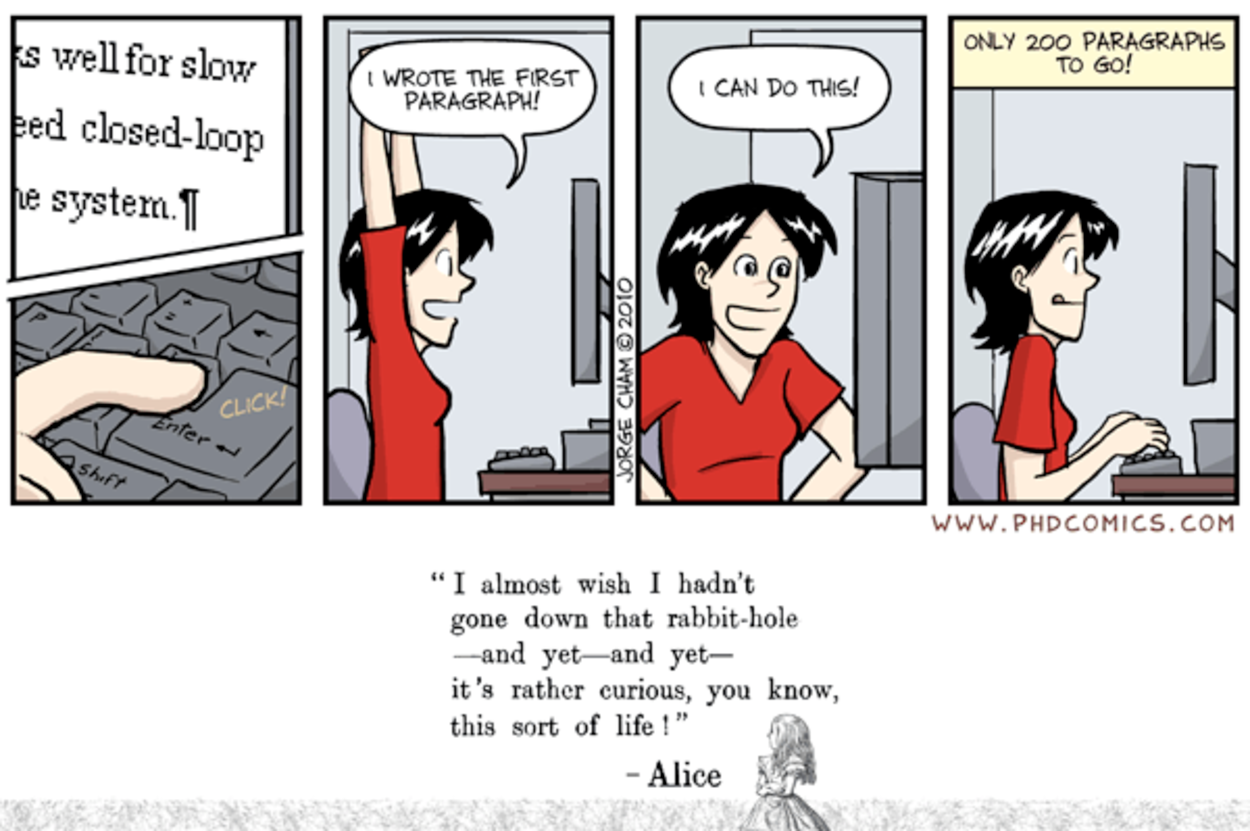
\includegraphics[width=\columnwidth,keepaspectratio,clip]{image_name.pdf}
\caption{\label{fig:image_label} Remember: relax and don't panic! (The image is from \cite{sample_bib_entry})}
 \end{center}
 \end{figure}

\pagestyle{empty}\pagestyle{fancy} %\conditionalblankpage \pagestyle{fancy}
\pagestyle{empty}
\fancyhead[LO]{\leftmark}   
\chapter*{Acknowledgements}
\pagestyle{fancy}

Acknowledge here (don't forget anyone!)
 %\conditionalblankpage

\renewcommand{\chaptermark}[1]{ \markboth{\appendixname \ \thechapter.\ #1}{}} 
\fancyhead[LO]{\leftmark}   %left portion of header on odd pages use ``\leftmark''

\bibliographystyle{unsrt}
\bibliography{thesis_bib.bib}
\end{document}
